
\documentclass{article}
\usepackage[fontset=fandol,UTF8]{ctex} 
\usepackage{iclr2027_conference}



\usepackage{amsmath,amsfonts,bm}

\newcommand{\figleft}{{\em (Left)}}
\newcommand{\figcenter}{{\em (Center)}}
\newcommand{\figright}{{\em (Right)}}
\newcommand{\figtop}{{\em (Top)}}
\newcommand{\figbottom}{{\em (Bottom)}}
\newcommand{\captiona}{{\em (a)}}
\newcommand{\captionb}{{\em (b)}}
\newcommand{\captionc}{{\em (c)}}
\newcommand{\captiond}{{\em (d)}}

\newcommand{\newterm}[1]{{\bf #1}}


\def\figref#1{figure~\ref{#1}}
\def\Figref#1{Figure~\ref{#1}}
\def\twofigref#1#2{figures \ref{#1} and \ref{#2}}
\def\quadfigref#1#2#3#4{figures \ref{#1}, \ref{#2}, \ref{#3} and \ref{#4}}
\def\secref#1{section~\ref{#1}}
\def\Secref#1{Section~\ref{#1}}
\def\twosecrefs#1#2{sections \ref{#1} and \ref{#2}}
\def\secrefs#1#2#3{sections \ref{#1}, \ref{#2} and \ref{#3}}
\def\eqref#1{equation~\ref{#1}}
\def\Eqref#1{Equation~\ref{#1}}
\def\plaineqref#1{\ref{#1}}
\def\chapref#1{chapter~\ref{#1}}
\def\Chapref#1{Chapter~\ref{#1}}
\def\rangechapref#1#2{chapters\ref{#1}--\ref{#2}}
\def\algref#1{algorithm~\ref{#1}}
\def\Algref#1{Algorithm~\ref{#1}}
\def\twoalgref#1#2{algorithms \ref{#1} and \ref{#2}}
\def\Twoalgref#1#2{Algorithms \ref{#1} and \ref{#2}}
\def\partref#1{part~\ref{#1}}
\def\Partref#1{Part~\ref{#1}}
\def\twopartref#1#2{parts \ref{#1} and \ref{#2}}

\def\ceil#1{\lceil #1 \rceil}
\def\floor#1{\lfloor #1 \rfloor}
\def\1{\bm{1}}
\newcommand{\train}{\mathcal{D}}
\newcommand{\valid}{\mathcal{D_{\mathrm{valid}}}}
\newcommand{\test}{\mathcal{D_{\mathrm{test}}}}

\def\eps{{\epsilon}}


\def\reta{{\textnormal{$\eta$}}}
\def\ra{{\textnormal{a}}}
\def\rb{{\textnormal{b}}}
\def\rc{{\textnormal{c}}}
\def\rd{{\textnormal{d}}}
\def\re{{\textnormal{e}}}
\def\rf{{\textnormal{f}}}
\def\rg{{\textnormal{g}}}
\def\rh{{\textnormal{h}}}
\def\ri{{\textnormal{i}}}
\def\rj{{\textnormal{j}}}
\def\rk{{\textnormal{k}}}
\def\rl{{\textnormal{l}}}
\def\rn{{\textnormal{n}}}
\def\ro{{\textnormal{o}}}
\def\rp{{\textnormal{p}}}
\def\rq{{\textnormal{q}}}
\def\rr{{\textnormal{r}}}
\def\rs{{\textnormal{s}}}
\def\rt{{\textnormal{t}}}
\def\ru{{\textnormal{u}}}
\def\rv{{\textnormal{v}}}
\def\rw{{\textnormal{w}}}
\def\rx{{\textnormal{x}}}
\def\ry{{\textnormal{y}}}
\def\rz{{\textnormal{z}}}

\def\rvepsilon{{\mathbf{\epsilon}}}
\def\rvtheta{{\mathbf{\theta}}}
\def\rva{{\mathbf{a}}}
\def\rvb{{\mathbf{b}}}
\def\rvc{{\mathbf{c}}}
\def\rvd{{\mathbf{d}}}
\def\rve{{\mathbf{e}}}
\def\rvf{{\mathbf{f}}}
\def\rvg{{\mathbf{g}}}
\def\rvh{{\mathbf{h}}}
\def\rvu{{\mathbf{i}}}
\def\rvj{{\mathbf{j}}}
\def\rvk{{\mathbf{k}}}
\def\rvl{{\mathbf{l}}}
\def\rvm{{\mathbf{m}}}
\def\rvn{{\mathbf{n}}}
\def\rvo{{\mathbf{o}}}
\def\rvp{{\mathbf{p}}}
\def\rvq{{\mathbf{q}}}
\def\rvr{{\mathbf{r}}}
\def\rvs{{\mathbf{s}}}
\def\rvt{{\mathbf{t}}}
\def\rvu{{\mathbf{u}}}
\def\rvv{{\mathbf{v}}}
\def\rvw{{\mathbf{w}}}
\def\rvx{{\mathbf{x}}}
\def\rvy{{\mathbf{y}}}
\def\rvz{{\mathbf{z}}}

\def\erva{{\textnormal{a}}}
\def\ervb{{\textnormal{b}}}
\def\ervc{{\textnormal{c}}}
\def\ervd{{\textnormal{d}}}
\def\erve{{\textnormal{e}}}
\def\ervf{{\textnormal{f}}}
\def\ervg{{\textnormal{g}}}
\def\ervh{{\textnormal{h}}}
\def\ervi{{\textnormal{i}}}
\def\ervj{{\textnormal{j}}}
\def\ervk{{\textnormal{k}}}
\def\ervl{{\textnormal{l}}}
\def\ervm{{\textnormal{m}}}
\def\ervn{{\textnormal{n}}}
\def\ervo{{\textnormal{o}}}
\def\ervp{{\textnormal{p}}}
\def\ervq{{\textnormal{q}}}
\def\ervr{{\textnormal{r}}}
\def\ervs{{\textnormal{s}}}
\def\ervt{{\textnormal{t}}}
\def\ervu{{\textnormal{u}}}
\def\ervv{{\textnormal{v}}}
\def\ervw{{\textnormal{w}}}
\def\ervx{{\textnormal{x}}}
\def\ervy{{\textnormal{y}}}
\def\ervz{{\textnormal{z}}}

\def\rmA{{\mathbf{A}}}
\def\rmB{{\mathbf{B}}}
\def\rmC{{\mathbf{C}}}
\def\rmD{{\mathbf{D}}}
\def\rmE{{\mathbf{E}}}
\def\rmF{{\mathbf{F}}}
\def\rmG{{\mathbf{G}}}
\def\rmH{{\mathbf{H}}}
\def\rmI{{\mathbf{I}}}
\def\rmJ{{\mathbf{J}}}
\def\rmK{{\mathbf{K}}}
\def\rmL{{\mathbf{L}}}
\def\rmM{{\mathbf{M}}}
\def\rmN{{\mathbf{N}}}
\def\rmO{{\mathbf{O}}}
\def\rmP{{\mathbf{P}}}
\def\rmQ{{\mathbf{Q}}}
\def\rmR{{\mathbf{R}}}
\def\rmS{{\mathbf{S}}}
\def\rmT{{\mathbf{T}}}
\def\rmU{{\mathbf{U}}}
\def\rmV{{\mathbf{V}}}
\def\rmW{{\mathbf{W}}}
\def\rmX{{\mathbf{X}}}
\def\rmY{{\mathbf{Y}}}
\def\rmZ{{\mathbf{Z}}}

\def\ermA{{\textnormal{A}}}
\def\ermB{{\textnormal{B}}}
\def\ermC{{\textnormal{C}}}
\def\ermD{{\textnormal{D}}}
\def\ermE{{\textnormal{E}}}
\def\ermF{{\textnormal{F}}}
\def\ermG{{\textnormal{G}}}
\def\ermH{{\textnormal{H}}}
\def\ermI{{\textnormal{I}}}
\def\ermJ{{\textnormal{J}}}
\def\ermK{{\textnormal{K}}}
\def\ermL{{\textnormal{L}}}
\def\ermM{{\textnormal{M}}}
\def\ermN{{\textnormal{N}}}
\def\ermO{{\textnormal{O}}}
\def\ermP{{\textnormal{P}}}
\def\ermQ{{\textnormal{Q}}}
\def\ermR{{\textnormal{R}}}
\def\ermS{{\textnormal{S}}}
\def\ermT{{\textnormal{T}}}
\def\ermU{{\textnormal{U}}}
\def\ermV{{\textnormal{V}}}
\def\ermW{{\textnormal{W}}}
\def\ermX{{\textnormal{X}}}
\def\ermY{{\textnormal{Y}}}
\def\ermZ{{\textnormal{Z}}}

\def\vzero{{\bm{0}}}
\def\vone{{\bm{1}}}
\def\vmu{{\bm{\mu}}}
\def\vtheta{{\bm{\theta}}}
\def\va{{\bm{a}}}
\def\vb{{\bm{b}}}
\def\vc{{\bm{c}}}
\def\vd{{\bm{d}}}
\def\ve{{\bm{e}}}
\def\vf{{\bm{f}}}
\def\vg{{\bm{g}}}
\def\vh{{\bm{h}}}
\def\vi{{\bm{i}}}
\def\vj{{\bm{j}}}
\def\vk{{\bm{k}}}
\def\vl{{\bm{l}}}
\def\vm{{\bm{m}}}
\def\vn{{\bm{n}}}
\def\vo{{\bm{o}}}
\def\vp{{\bm{p}}}
\def\vq{{\bm{q}}}
\def\vr{{\bm{r}}}
\def\vs{{\bm{s}}}
\def\vt{{\bm{t}}}
\def\vu{{\bm{u}}}
\def\vv{{\bm{v}}}
\def\vw{{\bm{w}}}
\def\vx{{\bm{x}}}
\def\vy{{\bm{y}}}
\def\vz{{\bm{z}}}

\def\evalpha{{\alpha}}
\def\evbeta{{\beta}}
\def\evepsilon{{\epsilon}}
\def\evlambda{{\lambda}}
\def\evomega{{\omega}}
\def\evmu{{\mu}}
\def\evpsi{{\psi}}
\def\evsigma{{\sigma}}
\def\evtheta{{\theta}}
\def\eva{{a}}
\def\evb{{b}}
\def\evc{{c}}
\def\evd{{d}}
\def\eve{{e}}
\def\evf{{f}}
\def\evg{{g}}
\def\evh{{h}}
\def\evi{{i}}
\def\evj{{j}}
\def\evk{{k}}
\def\evl{{l}}
\def\evm{{m}}
\def\evn{{n}}
\def\evo{{o}}
\def\evp{{p}}
\def\evq{{q}}
\def\evr{{r}}
\def\evs{{s}}
\def\evt{{t}}
\def\evu{{u}}
\def\evv{{v}}
\def\evw{{w}}
\def\evx{{x}}
\def\evy{{y}}
\def\evz{{z}}

\def\mA{{\bm{A}}}
\def\mB{{\bm{B}}}
\def\mC{{\bm{C}}}
\def\mD{{\bm{D}}}
\def\mE{{\bm{E}}}
\def\mF{{\bm{F}}}
\def\mG{{\bm{G}}}
\def\mH{{\bm{H}}}
\def\mI{{\bm{I}}}
\def\mJ{{\bm{J}}}
\def\mK{{\bm{K}}}
\def\mL{{\bm{L}}}
\def\mM{{\bm{M}}}
\def\mN{{\bm{N}}}
\def\mO{{\bm{O}}}
\def\mP{{\bm{P}}}
\def\mQ{{\bm{Q}}}
\def\mR{{\bm{R}}}
\def\mS{{\bm{S}}}
\def\mT{{\bm{T}}}
\def\mU{{\bm{U}}}
\def\mV{{\bm{V}}}
\def\mW{{\bm{W}}}
\def\mX{{\bm{X}}}
\def\mY{{\bm{Y}}}
\def\mZ{{\bm{Z}}}
\def\mBeta{{\bm{\beta}}}
\def\mPhi{{\bm{\Phi}}}
\def\mLambda{{\bm{\Lambda}}}
\def\mSigma{{\bm{\Sigma}}}

\DeclareMathAlphabet{\mathsfit}{\encodingdefault}{\sfdefault}{m}{sl}

\newcommand{\tens}[1]{\bm{\mathsfit{#1}}}
\def\tA{{\tens{A}}}
\def\tB{{\tens{B}}}
\def\tC{{\tens{C}}}
\def\tD{{\tens{D}}}
\def\tE{{\tens{E}}}
\def\tF{{\tens{F}}}
\def\tG{{\tens{G}}}
\def\tH{{\tens{H}}}
\def\tI{{\tens{I}}}
\def\tJ{{\tens{J}}}
\def\tK{{\tens{K}}}
\def\tL{{\tens{L}}}
\def\tM{{\tens{M}}}
\def\tN{{\tens{N}}}
\def\tO{{\tens{O}}}
\def\tP{{\tens{P}}}
\def\tQ{{\tens{Q}}}
\def\tR{{\tens{R}}}
\def\tS{{\tens{S}}}
\def\tT{{\tens{T}}}
\def\tU{{\tens{U}}}
\def\tV{{\tens{V}}}
\def\tW{{\tens{W}}}
\def\tX{{\tens{X}}}
\def\tY{{\tens{Y}}}
\def\tZ{{\tens{Z}}}


\def\gA{{\mathcal{A}}}
\def\gB{{\mathcal{B}}}
\def\gC{{\mathcal{C}}}
\def\gD{{\mathcal{D}}}
\def\gE{{\mathcal{E}}}
\def\gF{{\mathcal{F}}}
\def\gG{{\mathcal{G}}}
\def\gH{{\mathcal{H}}}
\def\gI{{\mathcal{I}}}
\def\gJ{{\mathcal{J}}}
\def\gK{{\mathcal{K}}}
\def\gL{{\mathcal{L}}}
\def\gM{{\mathcal{M}}}
\def\gN{{\mathcal{N}}}
\def\gO{{\mathcal{O}}}
\def\gP{{\mathcal{P}}}
\def\gQ{{\mathcal{Q}}}
\def\gR{{\mathcal{R}}}
\def\gS{{\mathcal{S}}}
\def\gT{{\mathcal{T}}}
\def\gU{{\mathcal{U}}}
\def\gV{{\mathcal{V}}}
\def\gW{{\mathcal{W}}}
\def\gX{{\mathcal{X}}}
\def\gY{{\mathcal{Y}}}
\def\gZ{{\mathcal{Z}}}

\def\sA{{\mathbb{A}}}
\def\sB{{\mathbb{B}}}
\def\sC{{\mathbb{C}}}
\def\sD{{\mathbb{D}}}
\def\sF{{\mathbb{F}}}
\def\sG{{\mathbb{G}}}
\def\sH{{\mathbb{H}}}
\def\sI{{\mathbb{I}}}
\def\sJ{{\mathbb{J}}}
\def\sK{{\mathbb{K}}}
\def\sL{{\mathbb{L}}}
\def\sM{{\mathbb{M}}}
\def\sN{{\mathbb{N}}}
\def\sO{{\mathbb{O}}}
\def\sP{{\mathbb{P}}}
\def\sQ{{\mathbb{Q}}}
\def\sR{{\mathbb{R}}}
\def\sS{{\mathbb{S}}}
\def\sT{{\mathbb{T}}}
\def\sU{{\mathbb{U}}}
\def\sV{{\mathbb{V}}}
\def\sW{{\mathbb{W}}}
\def\sX{{\mathbb{X}}}
\def\sY{{\mathbb{Y}}}
\def\sZ{{\mathbb{Z}}}

\def\emLambda{{\Lambda}}
\def\emA{{A}}
\def\emB{{B}}
\def\emC{{C}}
\def\emD{{D}}
\def\emE{{E}}
\def\emF{{F}}
\def\emG{{G}}
\def\emH{{H}}
\def\emI{{I}}
\def\emJ{{J}}
\def\emK{{K}}
\def\emL{{L}}
\def\emM{{M}}
\def\emN{{N}}
\def\emO{{O}}
\def\emP{{P}}
\def\emQ{{Q}}
\def\emR{{R}}
\def\emS{{S}}
\def\emT{{T}}
\def\emU{{U}}
\def\emV{{V}}
\def\emW{{W}}
\def\emX{{X}}
\def\emY{{Y}}
\def\emZ{{Z}}
\def\emSigma{{\Sigma}}

\newcommand{\etens}[1]{\mathsfit{#1}}
\def\etLambda{{\etens{\Lambda}}}
\def\etA{{\etens{A}}}
\def\etB{{\etens{B}}}
\def\etC{{\etens{C}}}
\def\etD{{\etens{D}}}
\def\etE{{\etens{E}}}
\def\etF{{\etens{F}}}
\def\etG{{\etens{G}}}
\def\etH{{\etens{H}}}
\def\etI{{\etens{I}}}
\def\etJ{{\etens{J}}}
\def\etK{{\etens{K}}}
\def\etL{{\etens{L}}}
\def\etM{{\etens{M}}}
\def\etN{{\etens{N}}}
\def\etO{{\etens{O}}}
\def\etP{{\etens{P}}}
\def\etQ{{\etens{Q}}}
\def\etR{{\etens{R}}}
\def\etS{{\etens{S}}}
\def\etT{{\etens{T}}}
\def\etU{{\etens{U}}}
\def\etV{{\etens{V}}}
\def\etW{{\etens{W}}}
\def\etX{{\etens{X}}}
\def\etY{{\etens{Y}}}
\def\etZ{{\etens{Z}}}

\newcommand{\pdata}{p_{\rm{data}}}
\newcommand{\ptrain}{\hat{p}_{\rm{data}}}
\newcommand{\Ptrain}{\hat{P}_{\rm{data}}}
\newcommand{\pmodel}{p_{\rm{model}}}
\newcommand{\Pmodel}{P_{\rm{model}}}
\newcommand{\ptildemodel}{\tilde{p}_{\rm{model}}}
\newcommand{\pencode}{p_{\rm{encoder}}}
\newcommand{\pdecode}{p_{\rm{decoder}}}
\newcommand{\precons}{p_{\rm{reconstruct}}}

\newcommand{\laplace}{\mathrm{Laplace}} 

\newcommand{\E}{\mathbb{E}}
\newcommand{\Ls}{\mathcal{L}}
\newcommand{\R}{\mathbb{R}}
\newcommand{\emp}{\tilde{p}}
\newcommand{\lr}{\alpha}
\newcommand{\reg}{\lambda}
\newcommand{\rect}{\mathrm{rectifier}}
\newcommand{\softmax}{\mathrm{softmax}}
\newcommand{\sigmoid}{\sigma}
\newcommand{\softplus}{\zeta}
\newcommand{\KL}{D_{\mathrm{KL}}}
\newcommand{\Var}{\mathrm{Var}}
\newcommand{\standarderror}{\mathrm{SE}}
\newcommand{\Cov}{\mathrm{Cov}}
\newcommand{\normlzero}{L^0}
\newcommand{\normlone}{L^1}
\newcommand{\normltwo}{L^2}
\newcommand{\normlp}{L^p}
\newcommand{\normmax}{L^\infty}

\newcommand{\parents}{Pa} 

\DeclareMathOperator*{\argmax}{arg\,max}
\DeclareMathOperator*{\argmin}{arg\,min}

\DeclareMathOperator{\sign}{sign}
\DeclareMathOperator{\Tr}{Tr}
\let\ab\allowbreak


\usepackage{hyperref}
\usepackage{url}
\usepackage{amssymb}
\usepackage{graphicx}
\usepackage{float}
\usepackage{bm} 
\usepackage{colortbl}
\usepackage{array}
\usepackage[nameinlink]{cleveref}
\DeclareRobustCommand{\parenCref}[1]{%
  (\hyperref[#1]{\nameCref{#1}~\ref*{#1}})%
}
\hypersetup{colorlinks, linkcolor={red!65!black}, citecolor={blue!75!black}, urlcolor={blue!75!black}}
\usepackage{cancel}
\usepackage{tcolorbox}
\usepackage{listings}
\usepackage{inconsolata}
\definecolor{codekeyword}{HTML}{008000}
\definecolor{codename}{HTML}{0000FF}
\definecolor{codecomment}{HTML}{3D7B7B}
\definecolor{codestring}{HTML}{BA2121}
\definecolor{codeoperator}{HTML}{666666}
\lstdefinestyle{python}{
    language=Python,
    basicstyle=\fontsize{8.4pt}{10pt}\selectfont\ttfamily,
    keywordstyle=\color{codekeyword}\bfseries,
    keywordstyle=[2]\color{codekeyword},
    deletekeywords=[2]{sum},
    emph={score_centering_loss},
    emphstyle=\color{codename},
    morekeywords=[3]{jax,numpy,lax},
    keywordstyle=[3]\color{codename}\bfseries,
    commentstyle=\color{codecomment}\itshape,
    stringstyle=\color{codestring},
    literate=*
        {0}{{\textcolor{codeoperator}{0}}}1
        {1}{{\textcolor{codeoperator}{1}}}1
        {2}{{\textcolor{codeoperator}{2}}}1
        {3}{{\textcolor{codeoperator}{3}}}1
        {4}{{\textcolor{codeoperator}{4}}}1
        {5}{{\textcolor{codeoperator}{5}}}1
        {6}{{\textcolor{codeoperator}{6}}}1
        {7}{{\textcolor{codeoperator}{7}}}1
        {8}{{\textcolor{codeoperator}{8}}}1
        {9}{{\textcolor{codeoperator}{9}}}1
        {=}{{\textcolor{codeoperator}{=}}}1
        {+}{{\textcolor{codeoperator}{+}}}1
        {-}{{\textcolor{codeoperator}{-}}}1
        {*}{{\textcolor{codeoperator}{*}}}1
        {/}{{\textcolor{codeoperator}{/}}}1,
    backgroundcolor=\color{gray!6},
    frame=single,
    rulecolor=\color{gridline},
    framesep=6pt,
    xleftmargin=6pt,
    xrightmargin=6pt,
    showstringspaces=false,
    columns=fullflexible,
    keepspaces=true,
    upquote=true,
    tabsize=4,
    breaklines=false
}

\newtcolorbox{notationbox}{colback=gridgray, colframe=gridgray, boxrule=0pt, arc=2pt, left=6pt, right=6pt, top=4pt, bottom=4pt, boxsep=0pt}
\definecolor{gentlelilac}{RGB}{112,48,175}
\renewcommand{\CancelColor}{\color{gentlelilac}}

\title{得分中心化稳定了异策略强化学习}

\author{Martin Marek \& Max Ryabinin \\
Together AI \\
\vspace{-8mm}
}

\newcommand{\fix}{\marginpar{FIX}}
\newcommand{\new}{\marginpar{NEW}}
\definecolor{gridblue}{RGB}{235,244,250}
\definecolor{gridcyan}{RGB}{234,247,247}
\definecolor{gridgreen}{RGB}{238,247,238}
\definecolor{gridamber}{RGB}{252,246,229}
\definecolor{gridorange}{RGB}{252,240,229}
\definecolor{gridyellow}{RGB}{250,248,225}
\definecolor{gridred}{RGB}{252,238,238}
\definecolor{gridteal}{RGB}{232,247,241}
\definecolor{gridpurple}{RGB}{246,239,250}
\definecolor{gridpink}{RGB}{251,237,246}
\definecolor{gridgray}{RGB}{243,243,243}
\definecolor{deep0}{HTML}{4C72B0}      
\definecolor{deep1}{HTML}{DD8452}
\definecolor{deep2}{HTML}{55A868}
\definecolor{tblteal}{HTML}{2A9D8F}   
\definecolor{figother}{HTML}{666666}  
\definecolor{gridline}{RGB}{210,210,210}
\definecolor{driftcoral}{HTML}{C65D4A}
\definecolor{signalteal}{HTML}{087F78}
\definecolor{equationnavy}{HTML}{283348}

\iclrfinalcopy 
\begin{document}


\vspace*{-5mm} 
\maketitle

\begin{abstract}
大型语言模型的强化学习（RL）对训练与推理引擎之间的微小差异极为敏感，这种现象通常被称为训练-推理不匹配（TIM）。  
然而，完全消除TIM是不切实际的，因为这将带来巨大的回放效率损失。  
在本文中，我们表明，在TIM存在的情况下，RL的不稳定性主要由\textit{漂移}引起：一种训练与推理引擎之间持续存在的偏差，且随着每一步训练不断累积。  
我们推导出一个加性的\textit{“得分中心化”}修正项，该修正项通过抵消漂移来稳定TIM下的强化学习。  
在从0.6B到30B参数的模型训练中，仅使用得分中心化的方法在量化条件下即可达到或超越基于重要性采样的方法，且当不匹配程度加剧时，性能差距进一步扩大。  
由于该修正为加性形式，得分中心化可与重要性采样相结合——在我们的延迟实验中，两者的组合表现优于纯重要性采样基准。
\end{abstract}

\begin{figure}[H]
    \centering
    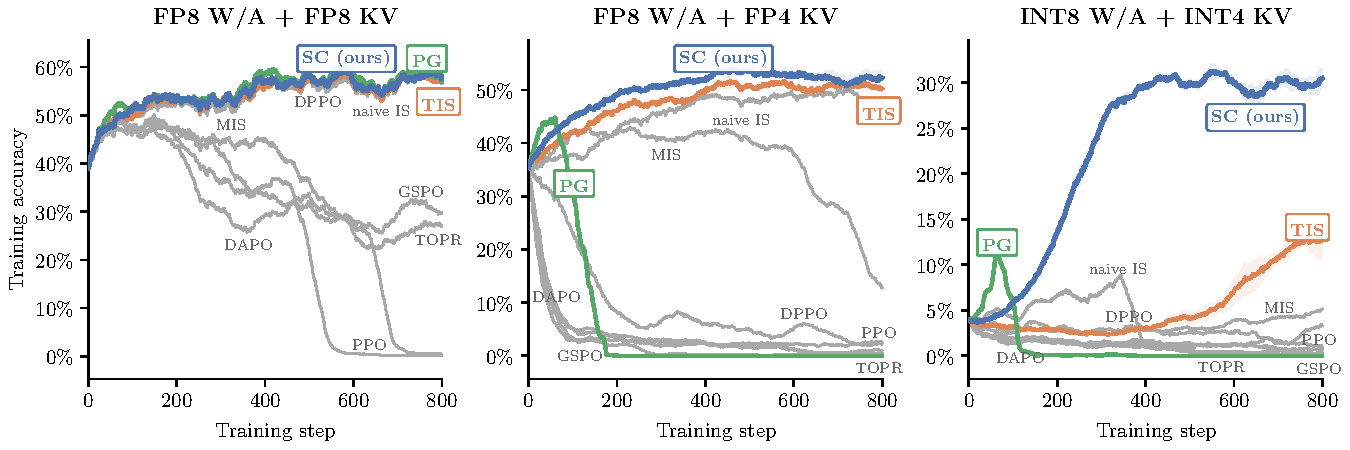
\includegraphics[width=1\linewidth]{plots/30b_math.pdf}
    \caption{
    \textbf{得分中心化在重度量化下优于重要性采样。}
我们使用强化学习在INTELLECT-2数学数据~\citep{intellect2}上对Qwen3-30B-A3B-Base~\citep{qwen3}进行训练，逐步增加采样器的量化强度。
我们在一个共享目标(\Cref{sec:results_setup})上比较修正规则。
在轻度量化情况下，朴素的\textcolor{deep2}{策略梯度（PG）}在800步内训练稳定，表现与修正方法相当。
随着量化严重程度的增加，训练变得越来越不稳定，且\textcolor{deep0}{得分中心化（SC）}、\textcolor{deep1}{截断重要性采样（TIS）}以及\textcolor{figother}{其他修正方法}之间的差距逐渐扩大。
    }
    \vspace{12pt}
    \label{fig:30b_math}
\end{figure}

\section{引言}

强化学习是当今大型语言模型训练中的关键步骤，这体现在越来越多的训练算力被分配给强化学习~\citep{o1,deepseek_r1,scaleRL,mai_1}。  
这通常通过PPO、GRPO、DAPO和IcePop等算法实现~\citep{ppo,grpo,dapo,icepop}，这些算法均基于策略梯度方法~\citep{reinforce}。

通过策略梯度进行大模型的训练包含采样轨迹、为每条轨迹分配奖励，并对加权轨迹计算梯度。  
更正式地，策略梯度方法将策略 $p_\theta$  在轨迹 $y$  上的期望奖励梯度计算为由奖励 $R$  加权的期望得分：
\begin{equation}
\nabla_\theta \, \mathbb{E}_{p_\theta}[R] = \mathbb{E}_{p_\theta} \big[ R \, \underbrace{\nabla_\theta \log p_\theta(y)}_{\text{``score''}} \big].
\label{eq:policy_grad}
\end{equation}

对从业者而言，计算公式\Cref{eq:policy_grad}右侧需要对模型进行两次独立的前向传播：第一次是采样器（推理引擎）的前向传播以生成轨迹，第二次是训练器的前向传播以计算生成轨迹上的梯度。  
理论上，训练器和采样器代表的是同一个模型，因此它们的输出应当完全相同。  
然而在实践中，这种情况很少发生。  
大多数强化学习代码库中，训练引擎与推理引擎之间存在微小的数值差异，导致所谓的“训练-推理不匹配”（TIM），这可能会降低训练性能\citep{scaleRL}，甚至引发奖励完全崩溃\citep{flashrl}。相比之下，监督微调通常使用来自不同模型或人工标注者的样本，具有稳定的训练动态，无需任何调整。

在本工作中，我们研究了强化学习对训练-推理不匹配敏感性的原因。通过分析策略梯度更新，我们发现其包含一个\textit{漂移}项，该项仅在训练策略与采样策略一致时为0。基于这一发现，我们提出了一种新的方法，用于在TIM条件下稳定强化学习的训练过程，称为\textbf{得分中心化}。\footnote{\href{https://github.com/martin-marek/score-centering}{\texttt{github.com/martin-marek/score-centering}}}
在使用Qwen3-0.6B进行Countdown实验以及使用Qwen3-30B-A3B-Base在INTELLECT-2数据集的数学子集上的实验中，我们展示了得分中心化方法能够达到或超越基于重要性采样的最先进训练稳定性技术。由于两种方法具有正交性，得分中心化可与重要性采样结合，以获得进一步的提升。

\section{背景与相关工作}
\label{sec:background}

\subsection{训练与推理不匹配的来源}

\Cref{eq:policy_grad} 中的原始策略梯度恒等式仅在用于计算梯度的策略与生成轨迹的策略相同时才成立。  
然而，在实际应用中，轨迹由 \textbf{采样器 $\bm{q_\theta}$ } 生成，而梯度则通过 \textbf{训练器 $\bm{p_\theta}$ } 计算。  
因此，当 $q_\theta \ne p_\theta$ 时会出现训练-推理不匹配问题。

TIM 的来源有很多，每种来源的严重程度各不相同。最严重的情况下，训练引擎和推理引擎以不同的精度运行，或基于两个独立的代码库，每个代码库都可能存在不同（难以检测）的错误，从而导致输出存在细微差异 \citep{speed_kills_stability, flashinfer_sentinel}。  
在较轻微的情况下，即使两个引擎都是正确的，并且使用相同的 GPU 内核，由于浮点运算的非结合性，仍可能产生不同的输出。\footnote{例如，在 \texttt{fp4\_e2m1} 精度下，$(0.5+0.5)+2=3$ ，但 $0.5+(0.5+2)=2$ 。}
由于采样是自回归的，而训练通常在序列维度上并行化，训练和推理引擎可能会以不同的输入形状调用相同的内核，从而改变归约的顺序，导致微小的浮点差异。  
批量不变内核消除了对输入形状的依赖，但需要大量的工程工作，并导致GPU利用率下降 \citep{thinky_nondeterminism}。  
将两个引擎的精度从bf16切换到fp16也能显著减少不匹配 \citep{fp16_rl}，但无法完全消除。

最后，即使训练器和生成器使用相同的批量不变内核，由于更新延迟仍可能导致TIM的发生。  
在强化学习中实现高GPU利用率需要解耦训练与推理引擎，异步运行它们 \citep{areal}，并通过连续批量处理回放数据 \citep{orca}。  
这意味着单个训练批次，甚至单个回放序列的不同子序列，都可能来自不同的模型检查点 \citep{pipelineRL}。  
在长上下文环境（如Agentic编程）中，延迟问题尤为严重，某些回合可能在几分钟内完成，而其他回合则可能持续数小时甚至数天 \citep{single_rollout}。  
从硬件利用率的角度来看，算法性地稳定使用过时回放数据的训练过程，比试图完全消除延迟更为可取 \citep{areal}。

我们的目标是提出一种在TIM下的稳定强化学习训练方法，以实现高硬件利用率的同时确保训练的稳定性。

\subsection{重要性采样修正}

假设在 \Cref{eq:policy_grad} 中，轨迹来自采样器 $q_\theta$，而非训练器 $p_\theta$，其中 $q_\theta \ne p_\theta$。那么我们可以使用重要性采样（IS）确切地纠正训练-推理不匹配：
\begin{equation}
\nabla_\theta \, \mathbb{E}_{p_\theta}[R] = \mathbb{E}_{p_\theta} \left[ R \, \nabla_\theta \log p_\theta(y) \right] = \mathbb{E}_{q_\theta} \left[ \frac{p_\theta(y)}{q_\theta(y)} R \, \nabla_\theta \log p_\theta(y) \right].
\label{eq:policy_grad_is}
\end{equation}
\Cref{eq:policy_grad_is} 适用于完整序列；在实际应用中，该比例通常按每个 \citep{gspo} 应用。无论哪种方式，重要性采样都会修正 TIM，但代价是方差增加。加权得分会乘以重要性比例 $r = \frac{p_\theta(y)}{q_\theta(y)}$，该比例在罕见的 \citep{gspo} 上可能取任意大的值，从而放大梯度估计的方差 \citep{ionides, owen_mc}。由于使用原始的重要性比例进行训练不稳定，实践中采用的方法会对重要性比例进行限制，这不可避免地引入了偏差。

\Cref{tab:is_methods}（在 \Cref{sec:is_methods} 中）表明，大多数流行的修正方法基于重要性采样，并落在一个简单的网格上，其具体形式取决于重要性比率被截断或掩码的区域。一个显著的异常值是 DPPO，它使用基于二值总变差的掩码区域——但其目标函数仍然使用重要性采样比率，与其他网格中的所有方法一样。超越表格范围，\citet{alp} 将可学习的扰动注入训练器的隐状态，并将扰动后的策略作为重要性比率的分子——通过减少比率的重尾而非截断来改进——但仍依赖于重要性采样。相比之下，\textit{得分中心化}（我们在 \Cref{sec:sc} 中提出的方法）完全不使用重要性比率、不进行掩码、也不进行截断——它是一个加性修正项，从根本上区别于该网格中的每一种方法。


\section{为什么强化学习对偏差敏感}
\label{sec:diagnosis}

要理解为什么强化学习（RL）对TIM如此敏感，有助于我们理解强化学习与监督微调（SFT）之间的差异。正如我们之前所指出的，即使在训练数据完全由另一个模型离线生成且没有任何重要性采样修正的情况下，SFT仍然保持稳定~\citep{distillation, deepseek_r1}。换句话说，SFT对过时性或内核选择完全不敏感。

至关重要的是，当优势值为 $+1/0$ 时（即奖励未进行中心化或规范化），且训练完全离线（即采样器从未更新），策略梯度在具有二元奖励的任务上退化为 SFT。\footnote{在实际应用中，优势值几乎总是包含负值（例如，由于组中心化 \citep{grpo}），即使训练允许一定程度的延迟，也从不是完全离线的。} 因此，我们可以认为 \textbf{奖励模式} 和 \textbf{延迟性} 是 SFT 与 RL 之间的两个关键差异。\footnote{注意，将奖励平移一个常数不会改变同策略下的期望梯度，而组中心化仅对一组 $G$  回合的奖励进行缩放，缩放因子为 $1 - 1/G$ —— 中心化奖励的原因是它能降低梯度方差 \citep{greensmith, dr_grpo}。  
然而，在异策略情况下这不成立：使用 $+1/0$  的 SFT 收敛到极大似然估计量 \citep{bishop}，而使用 $0/-1$  奖励的 SFT 是退化的：损失会无界增长，可能导致模型坍塌 \citep{finetuning_dynamics}。} 
我们想要确定这两种机制中，哪一种会导致对TIM的敏感性增加。

我们通过一个简单的训练设置来测试这一点，该设置包含有意的策略不匹配。我们对 Qwen3-1.7B \citep{qwen3} 在 Countdown \citep{stream_of_search} 上进行训练，并人为地将采样器的权重与训练器的权重相比进行微小扰动，以创建受控的 TIM。我们在 \Cref{sec:results} 中进一步说明了该设置的理由，并测试了更现实的 TIM 来源。



\begin{figure}[H]
    \centering
    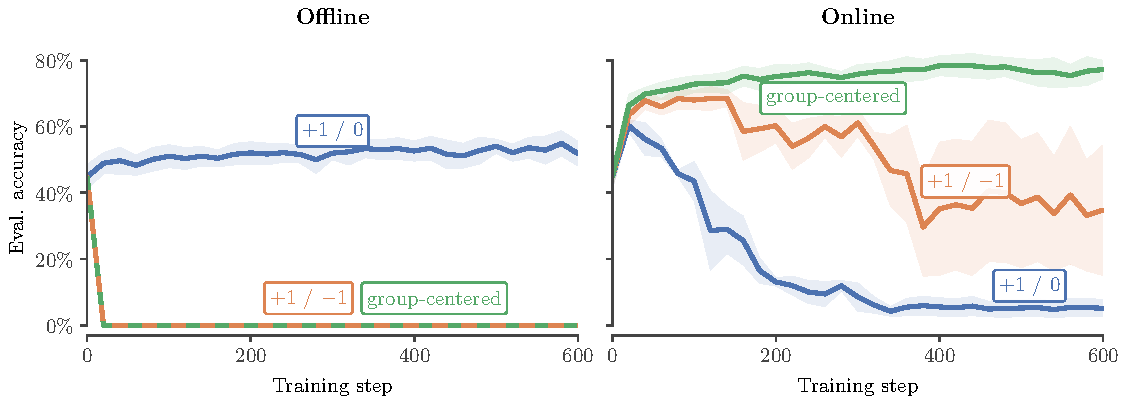
\includegraphics[width=0.9\linewidth]{plots/2b_online_vs_offline.pdf}
    \caption{Qwen3-1.7B 在 Countdown 上三种奖励模式下的离线与在线训练对比。离线训练仅在 $+1/0$ 奖励下稳定，而在线训练在 TIM 模式下于 $+1/0$ 奖励时最不稳定。}
    \label{fig:2b_online_vs_offline}
\end{figure}

\Cref{fig:2b_online_vs_offline} 表明，在此设置下，离线训练仅在 $+1/0$（非负）奖励下稳定，而在线训练则相反——组中心奖励 \citep{grpo}，即组内混合正负值的奖励，是最稳定的，而 $+1/0$ 奖励——对离线训练最稳定——对在线训练却是最不稳定的。因此，我们假设存在两种分离的机制：一种导致离线训练中使用 \textit{负} 奖励时不稳定，另一种则导致在线训练中使用 \textit{正} 奖励时不稳定。

本文的主要关注点是在线强化学习，因此我们不再深入探讨离线训练中负奖励带来的不稳定性。\Citet{finetuning_dynamics} 认为这种不稳定性背后的主要机制在于负奖励的无界性与分布锐化相结合。对数概率从下方无界，因此在带有负奖励的离线训练过程中，它们可能发散至 $-\infty$。这种现象在在线训练中并不存在，因为在在线训练中仅会采样高概率的 token。  
这种不对称性已有充分记录：仅基于正例进行训练（即蒸馏或拒绝微调）即使在离线情况下也完全稳定 \citep{distillation, deepseek_r1}，而负梯度则可能降低正确响应的概率 \citep{nthr}——尽管是同策略的，它们仍携带了有用的学习信号 \citep{negative_reinforcement}。

在在线训练中，我们观察到的行为与离线训练相反——仅使用正向奖励的设置是\emph{最不稳定}的。因此我们假设，这种不稳定性必须源于训练过程的在线特性。
需要注意的是，在TIM下使用$+1/0$奖励进行在线训练本身也是一种蒸馏：训练器被拟合到采样器的成功轨迹上，而采样器是自身的一个有偏副本，其权重在每一步后都从训练器更新。与离线蒸馏唯一的不同在于教师会随着学生移动，因此不稳定性就来源于此。

\section{得分中心化}
\label{sec:sc}

\begin{notationbox}
\textbf{符号说明.} 从一次采样 $y$  的更新会对其所有 token 得分进行求和，每个得分按该采样的奖励（或优势）$R$ 加权。我们考察单个 token $y_t$ 在给定其前缀 $y_{<t}$ 条件下的期望贡献。采样器 $q$  生成 token $y_t$；$v$  表示词表的索引。$p_v$  和 $q_v$  分别是 $v$  在训练者 $p$  和采样器 $q$  下的下一个 token 概率，$s_v = \nabla_\theta \log p_v$  是其得分，$\bar{s} = \sum_v q_v \, s_v$  是采样器下的期望得分。$\mathbb{E}_q$  和 $\mathbb{E}_p$  对前缀之后的其余采样部分进行求和。
\end{notationbox}

考虑在具有恒定 $+1$  奖励的环境中使用原始策略梯度进行强化学习训练。理论上，应该没有学习发生——因为奖励是恒定的，所以环境没有提供任何“信号”。事实上，在同策略下，每个前缀的期望梯度都为零：$\mathbb{E}_p[R \, s_{y_t}] = R \, \mathbb{E}_p[s_{y_t}] = R \cdot 0$ ，因为 $\mathbb{E}_p[s_{y_t}] = \sum_v p_v \nabla_\theta \log p_v = \nabla_\theta \sum_v p_v = \nabla_\theta 1 = 0$ 对于任意分布都成立。

\clearpage
然而，在 TIM 下，期望梯度是非零的：token 从采样器 $q$ 中采样，而得分通过训练器 $p$ 计算，因此 $\bar{s} = \mathbb{E}_q[s_{y_t}] \ne 0$ 通常不为零。 \begingroup\color{equationnavy}
利用协方差恒等式，\footnote{$\mathrm{Cov}(A, B) = \mathbb{E}[AB] - \mathbb{E}[A]\,\mathbb{E}[B] \; \Rightarrow \; \mathbb{E}[AB] = \mathbb{E}[A]\,\mathbb{E}[B] + \mathrm{Cov}(A, B)$} 我们可以将前缀处的期望策略梯度更新分解为一个 \textcolor{driftcoral}{``漂移''} 项和一个 \textcolor{signalteal}{``信号''} 项：
\begin{equation}
\underbrace{\mathbb{E}_q[R \, s_{y_t}]}_{\text{policy gradient update}}
\hspace{-3mm} = \hspace{1.3mm} \textcolor{driftcoral}{\underbrace{\mathbb{E}_q[R] \; \bar{s}}_{\text{``drift''}}}
\; + \; \textcolor{signalteal}{\underbrace{\mathrm{Cov}_q(R, \; s_{y_t})}_{\text{``signal''}}}
\label{eq:drift}
\end{equation}
\endgroup
\vspace{-1mm}
\paragraph{漂移是TIM的一种伪影，表现为对采样器的蒸馏作用。} 漂移项不包含关于哪些轨迹成功的信息：它仅通过奖励的均值 $\mathbb{E}_q[R]$ 依赖于奖励。只有协方差项能观察到哪个 token 导致了哪个奖励。漂移项的作用实际上由其方向 $\bar{s}$ 决定：期望得分是交叉熵（SFT）损失相对于采样器作为教师时的负梯度，因此原始策略梯度在每个前缀处将训练器向采样器蒸馏，且缩放因子为该前缀处的期望奖励。这完全是 TIM 的一个结果：同策略下，训练器已与采样器匹配，因此 $\bar{s}=0$ ，漂移项消失。向一个固定的教师进行蒸馏是无害的——它会收敛至该教师的极大似然拟合。然而，采样器并非固定不变：它是训练器的一个有偏副本（例如量化或过时），因此每一步都会将训练器推向采样器；随后训练器权重被同步回采样器，误差在反馈环中累积而非收敛。这解释了为何在所有奖励为正的情况下进行在线训练是 \Cref{fig:2b_online_vs_offline} 中最不稳定的设置。\citet{probing} 同样指出系统性偏差是 TIM 下不稳定的根源，并表明这种偏差通过正反馈环不断放大。

\paragraph{组中心化不能消除漂移。} 组中心化 \citep{grpo} 使得在某个提示的轨迹中优势值之和为零，但在单个前缀上会出现漂移现象，且在给定前缀上的期望优势并不为零：一个很可能导向正确答案的前缀具有正的期望优势，而已经包含错误的前缀则具有负的期望优势。因此，漂移恰好出现在携带学习信号的前缀处——对于具有正期望优势的前缀，训练器会被拉向采样器；而对于具有负期望优势的前缀，训练器则被推离采样器，无论相关 token 是否影响奖励。组中心化相对于 $+1/0$ 奖励确实减小了漂移，这与它在 \Cref{fig:2b_online_vs_offline} 情景中是最稳定的在线设置相一致，但并未完全消除漂移。

\paragraph{得分中心化可消除漂移。} 这些观察结果直接促使我们提出方法，称为 \emph{得分中心化}：即使在 TIM 情况下，我们也希望每个前缀的期望得分都为零，如同策略时一样。我们只需从每个得分中减去采样器下的期望得分，将 $s_{y_t}$ 替换为中心化的得分 $\tilde{s}_{y_t}$ 即可：
\begin{equation}
\tilde{s}_{y_t} = s_{y_t} - \bar{s}.
\label{eq:sc}
\end{equation}
带得分中心化的期望策略梯度更新变为：
\begin{align}
\hspace{25mm} \mathbb{E}_q[R\,\tilde{s}_{y_t}] &= \overset{\color{gentlelilac} \mathbb{E}_q[\tilde{s}_{y_t}] \,=\, \bar{s} - \bar{s} \,=\, 0}{\cancel{\mathbb{E}_q[R]\;\mathbb{E}_q[\tilde{s}_{y_t}]}} + \mathrm{Cov}_q(R, \tilde{s}_{y_t}) \label{eq:sc_bias} \\
&= \mathrm{Cov}_q(R, \tilde{s}_{y_t}) \nonumber \\
&= \mathrm{Cov}_q(R, s_{y_t}) \;\; \longleftarrow \;\;
\smash[t]{\begin{array}{@{}l@{}}
\text{only difference to on-policy update} \\
\text{is the covariance sampling distribution}
\end{array}} \nonumber
\end{align}

定义在 \Cref{eq:sc} 中的中心化得分在采样器下具有零均值，因为两个期望都在同一分布下计算——即使在异策略情况下，漂移在每个前缀处也会被确切抵消。\Cref{eq:sc_bias} 表明，使用得分中心化的期望更新在至多分布差异的情况下等于同策略的期望更新——无论是同策略还是在重要性采样下的 TIM 情况，协方差都是在训练分布 $p_\theta$ 下测量的，而得分中心化则在采样分布 $q_\theta$ 下测量它。当不存在 TIM 时，即当 $p_\theta = q_\theta$ 时，得分中心化不起作用，因为 \Cref{eq:sc} 中的修正项恰好为零。

\paragraph{得分中心化与重要性采样。} 重要性采样与得分中心化一样，也能精确消除漂移。然而，重要性采样使用一个随机的乘性修正项，这意味着它会增加梯度方差，且其值依赖于所采样的 token。对于稀有 token，重要性比率可能非常大，因此几乎所有实际实现都会以某种方式对大的重要性比率进行截断或掩码处理 (\Cref{tab:is_methods})，从而重新引入漂移。相比之下，得分中心化是一种给定前缀时为 \textit{确定性} 的 \textit{加性} 修正项——它不依赖于所采样的 token，且可以精确计算。由于得分中心化和重要性采样以独立的方式纠正 TIM，这两种方法可以相互组合，如 \Cref{sec:is_composition} 所述。

\paragraph{与经典基准的关系。} 从策略梯度中减去一个均值为零的量是一种经典的方差减小思想：奖励基准 \citep{reinforce} 和得分函数控制变量 \citep{bbvi} 都基于恒等式 $\mathbb{E}_p[s_{y_t}] = 0$。得分中心化是一种偏差校正，而非方差减小：所减去的向量在给定前缀的情况下是确定性的，并被选择用来调整更新的均值，而同策略下的奖励基准仅改变方差而不改变均值。在异策略情况下，等于前缀处期望奖励（确切的价值函数）的奖励基准也会在期望上消除漂移；而得分中心化则无需评论员即可获得相同的期望更新。据我们所知，之前的方法从未减去期望得分本身：在同策略下其值为零，而在经典的异策略强化学习中，对动作空间的不可处理期望进行计算，因此异策略方法依赖重要性采样。在 TIM 框架下对大模型进行强化学习训练是不寻常的，因为期望得分既非零又可精确计算，即通过对下一个 token 的 logprob 求和得到。

\subsection{实施}
\label{sec:sc_impl}

存储采样器完整的下一个 token 分布开销过大。因此，我们仅记录其前 $k$ 个最高 logprob ($k=128$ )，并将尾部建模为经过缩放以匹配采样器尾部质量的训练器分布。我们通过标量损失实现得分中心化：
\begin{equation}
L = -R \, \Big( \log p_{y_t} - \sum_{v \in H} \operatorname{sg}\left[ q_v - \rho \, p_v \right] \log p_v \Big),
\label{eq:sc_loss_main}
\end{equation}
其中 $\rho$ 表示采样器与训练器尾部质量的比例，$\operatorname{sg}$ 表示停止梯度。在我们测试的每种情景下，使用 $k=128$ 或甚至 $k=32$ 都能实现完整的得分中心化（\Cref{sec:topk_ablation}）。下面的代码片段展示了一个单 token 的最小实现：
\begin{lstlisting}[style=python]
import jax.numpy as jnp
from jax.lax import stop_gradient

def score_centering_loss(train_logp, samp_logp, topk_ids, sampled_token, advantage):
    train_head_logp = train_logp[topk_ids]
    tail_mass_ratio = (1 - jnp.exp(samp_logp).sum()) / (1 - jnp.exp(train_head_logp).sum())
    head_prob_residual = jnp.exp(samp_logp) - tail_mass_ratio * jnp.exp(train_head_logp)
    logp_correction = (stop_gradient(head_prob_residual) * train_head_logp).sum()
    return -advantage * (train_logp[sampled_token] - logp_correction)
\end{lstlisting}

在 \Cref{sec:sc_implementation} 中，我们提供了得分中心化完整的推导过程以及支持重要性权重的泛化实现。


\section{实验}
\label{sec:results}

\subsection{设置}
\label{sec:results_setup}

我们对比了得分中心化方法与 \Cref{tab:is_methods} 中的修正方法，在 \citep{stream_of_search} 上训练 Qwen3-0.6B-Instruct，以及在 {INTELLECT-2} 数据集的数学子集 \citep{intellect2} 上训练 Qwen3-30B-A3B-Base。

\noindent\textbf{共享目标.} 现有方法通常将多种技术组合在一起：例如，DAPO 将非对称裁剪与动态采样 \citep{dapo} 结合，而 IcePop 将训练与推理引擎之间的 MIS 与策略版本间的 PPO 裁剪 \citep{icepop} 结合。为了单独比较每种修正方法，我们全程使用相同的目标（以组中心奖励为基准的 REINFORCE），并将每种修正方法单独应用于该目标之上。所有方法共享相同的采样器、训练器、优化器和优势函数，每个批量执行一次 SGD 步骤。所有重要性比率均使用采样器记录的概率。\Cref{tab:is_methods} 展示了修正规则和超参数，以及实现说明。学习率、批量大小和计算成本列于 \Cref{sec:experimental_details}。

\noindent\textbf{不匹配情景。} 通常情况下，我们难以找到自然的设置，使得TIM严重到能够在数小时的GPU训练时间内观察到表现最强的方法之间的统计显著差异。我们认为这是训练过程中漂移累积的结果（\Cref{sec:sc}）：在轻微的TIM下，需要更多的训练步数才能积累足够的漂移，而在漂移足够之前，表现最好的方法会重叠。我们在 \Cref{sec:results_weight_noise} 中展示了这一点：在较小的权重噪声下，表现最好的方法重叠，导致无法进行比较；而随着TIM的增加，方法更早崩溃，它们之间的性能差距也逐渐增大。由于我们无法负担在极长训练周期中对校正方法进行具有统计显著性的消融实验，因此我们故意放大TIM，将这些结果作为在较温和TIM下大规模训练的代理。出于这一原因，在 \Cref{sec:results_quant_stale} 中我们测试了故意严重的量化和延迟设置。值得注意的是，先前的工作对于强化学习在TIM下的实际不稳定性存在分歧：\citet{fp8_rl} 发现仅使用token级重要性采样且不匹配数值的情况下，fp8回放仍保持稳定；而 \citet{mai_1} 在尽力最小化TIM并使用bf16采样时，仍观察到训练发散。我们认为这两种发现都与训练过程中的漂移累积是一致的：要在短时间训练中观察到不稳定性，必须存在严重的TIM；而轻微的TIM同样可能导致训练不稳定，但需要更多训练步数才能显现。

\subsection{合成权重噪声}
\label{sec:results_weight_noise}

为了快速进行初步实验，我们发现研究通过向采样器的权重添加人工偏移量（相对于训练器的权重）所引起的TIM是有益的。具体而言，我们设置 $\theta_\textrm{sampler} = \theta_\textrm{trainer} \, + \, \Delta \theta$ ，其中 $\Delta \theta$ 在训练开始时从各向同性高斯分布中采样并固定不变。尽管这是我们在研究中采用的最不现实的设定，但它导致了最快的方法间坍缩与分离，并实现了TIM的连续变化尺度，使其成为初步实验中不可或缺的工具。

在 \Cref{fig:06b_weight_noise} 的三种噪声尺度下，我们发现得分中心化（SC）、截断重要性采样（TIS）和掩码重要性采样（MIS）表现最佳，以及它们的组合：MIS + SC 和 TIS + SC。  
我们在 \Cref{sec:is_composition} 中描述了如何将得分中心化与重要性采样方法结合。在最严重的噪声条件下，仅有得分中心化及其与 MIS 或 TIS 的组合能够稳定训练。\Cref{fig:06b_weight_noise} 还显示了训练过程中漂移的累积——崩溃的方法在噪声不匹配更大的情况下会更早崩溃。例如，DPPO 在三种噪声尺度下的崩溃点分别约为第 160、80 和 20 步，而 TIS 在最小噪声下能够稳定训练，但在较大的两种噪声下分别于约第 180 和 40 步崩溃。

\begin{figure}[H]
    \centering
    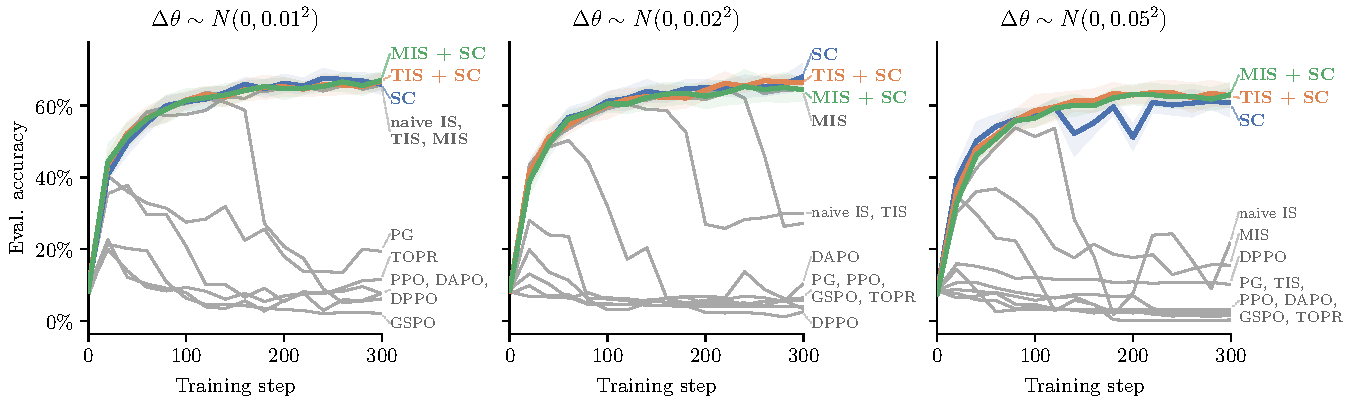
\includegraphics[width=\linewidth]{plots/06b_weight_noise.pdf}
    \caption{Qwen3-0.6B 在倒计时任务中，对采样器权重添加高斯噪声。噪声越大，越早发生坍缩。仅使用得分中心化（单独使用或与 TIS/MIS 结合）在最大噪声下仍能稳定训练。}
    \label{fig:06b_weight_noise}
\end{figure}

\subsection{量化与延迟}
\label{sec:results_quant_stale}

接下来，我们将人工权重噪声替换为两种更真实的TIM来源：量化和延迟。  
我们特意使这两种TIM来源都较为严重（\Cref{sec:results_setup}），以便在数百个训练步骤内，使用短序列长度观察不同修正方法之间的分离效果。  
在量化情景中，仅对采样器（权重、活性值和KV缓存）进行量化；而训练器使用bf16精度。  
延迟情景也故意设置得较为严重：推理引擎仅每64步更新一次，而非最大延迟为64步。  
实际上，更理想的做法是尽可能频繁地更新推理引擎（\citep{pipelineRL}），并为采样器和训练器采用相同的量化方案（\citep{jet_rl}）。

在量化采样情景（\Cref{fig:06b_quant_stale}）中，我们观察到与 \Cref{fig:06b_weight_noise} 类似的结果——仅使用得分中心化，或将其与 TIS / MIS 结合使用时表现最佳。然而，在延迟情景下，将得分中心化与 TIS / MIS 结合使用的表现最佳，优于原始的得分中心化方法。我们认为这是由于得分中心化衡量的是采样器而非训练器下的协方差 \parenCref{eq:sc_bias}：TIS 部分修正了采样分布，而得分中心化则消除了剩余的漂移。因此，当训练器在同步之间可能远离采样器时，我们建议将得分中心化与重要性采样校正结合使用。PPO 和 DAPO 在延迟情况下仍能维持性能，但在量化和权重噪声下会崩溃。这与它们的裁剪机制设计用于处理策略移动产生的比率一致：延迟会产生此类比率，而数值误差则不会。

\begin{figure}[H]
    \centering
    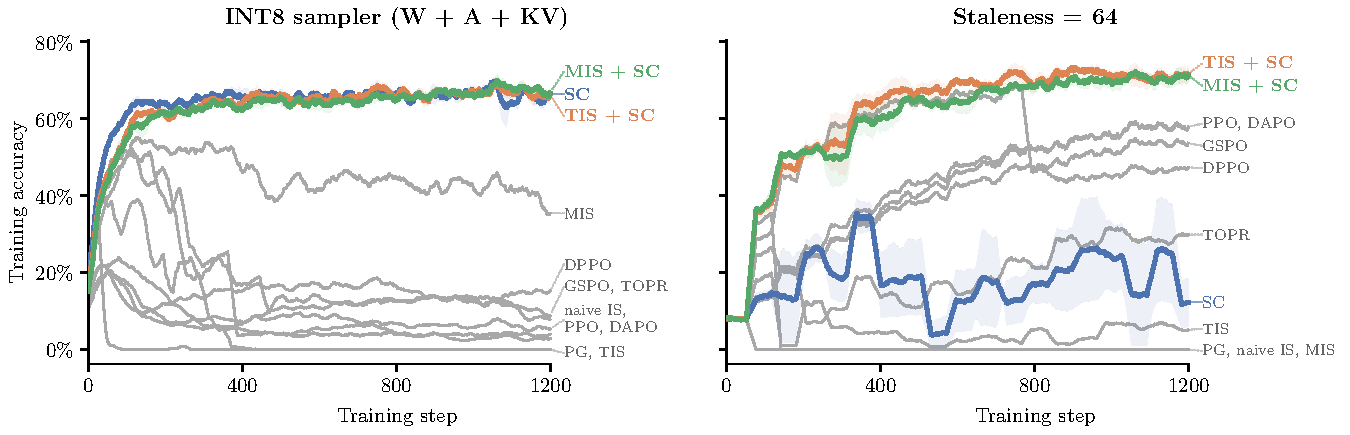
\includegraphics[width=\linewidth]{plots/06b_quant_stale.pdf}
    \caption{Qwen3-0.6B在倒计时任务中，左侧使用int8采样器，右侧使用每64步更新一次的采样器。在量化条件下，仅采用得分中心化和组合方法表现最佳；在过时性条件下，结合TIS/MIS的得分中心化组合方法占据主导地位。}
    \label{fig:06b_quant_stale}
\end{figure}

\subsection{缩放至300亿}
\label{sec:results_30b}

最后，我们通过在 INTELLECT-2 数学数据集上对 Qwen3-30B-A3B-Base 进行训练，并在采样器量化三个不同级别（\Cref{fig:30b_math}）下验证了我们的结果在更大规模下的有效性。由于 Qwen3-30B-A3B 是一个专家混合模型，采样器与训练器也可能在专家路由上产生分歧；我们未重放路由器索引，尽管在实际应用中这样做会更优 \citep{r3}。使用 FP8 采样器时，即使未经校正的策略梯度也能稳定训练，达到 $58\%$ 的训练准确率。当 KV 缓存被量化为 FP4 后，策略梯度在 200 步内崩溃，而 MIS 在训练后期才崩溃，而得分中心化（$52\%$）和 TIS（$51\%$）则保持稳定。使用 INT8 采样器和 INT4 KV 缓存时，得分中心化达到 $30\%$，TIS 达到 $12\%$，而其他所有方法均低于 $5\%$。



\section{结论}

本文做出了两项贡献。第一项是解释了为何大模型的强化学习训练对训练-推理不匹配（TIM）如此敏感。在TIM条件下，策略梯度更新包含一个漂移项，该漂移项起到了向采样器进行蒸馏的作用。由于采样器是训练器的一个有偏副本，并且周期性地同步回训练器，这种偏差会在反馈环中不断累积：TIM越严重，训练越早崩溃。先前的工作已经观察到这种偏差会随着训练过程不断累积 \citep{probing, mai_1}。我们证明，仅通过消除漂移项（无需重要性比例），即可在严重量化情况下稳定训练，这确立了漂移项是导致不稳定的根源。这也解释了为何从一个完全不同的模型进行离线蒸馏是稳定的，而在线强化学习却在微小数值差异下崩溃：关键并不在于不匹配的大小，而在于教师模型是否固定，还是追踪学生模型。

我们的第二个贡献是得分中心化，这是一种实用的方法，通过减去期望得分来消除漂移。它是一个无需超参数的加性修正项，可表示为标量损失 \parenCref{eq:sc_loss_main}，且能与重要性采样方法（如 TIS 和 MIS）组合使用。确切的得分中心化需要采样器完整的下一个 token 分布；因此，我们引入了一种近似方法，仅需采样器的 top-$k$  logprob 即可，且在所有实验中表现均与确切得分中心化相当 (\Cref{sec:topk_ablation})。在温和的 TIM 条件下，得分中心化与重要性采样方法表现相当；在严重量化情况下，它是唯一能够稳定训练的方法；而在严重延迟情况下，其与 TIS 或 MIS 的组合表现最佳。

\paragraph{局限性。} 得分中心化可以消除漂移，但剩余的更新衡量的是采样器而非训练器下的奖励与得分之间的协方差 \parenCref{eq:sc_bias}。在严重延迟的情况下，这种不匹配尤为关键，此时得分中心化与重要性采样结合时表现最佳 (\Cref{sec:results_quant_stale})。此外，我们的核心结果来自对短序列故意设置的严重不匹配，作为在较轻不匹配下进行长时间训练的代理。

\bibliography{paper.bib}
\bibliographystyle{iclr2027_conference}

\appendix
\clearpage


\section{实施得分中心化}
\label{sec:sc_implementation}

\begin{notationbox}
\textbf{符号}（如 \Cref{sec:sc} 所示）。在固定前缀下，$y_t$ 为采样得到的 token，$v$ 为词表中的 token；$p_v$、$q_v$ 分别为其训练器和采样器的概率，$s_v = \nabla_\theta \log p_v$ 为其得分，$\bar{s} = \sum_v q_v \, s_v$ 为采样器下的期望得分。
\end{notationbox}

\subsection{Top-$k$ 近似}

\textit{完整} 得分中心化，如我们迄今所描述的，对大多数实际应用而言成本过高。按照 \Cref{eq:sc} 所述，计算得分中心化校正项（即对采样器每个 token 分布的得分期望）需要存储每个采样 token 的完整输出 logprobs。例如，Qwen3 模型的词表大小为 152K，仅以 fp32 精度存储单个 token 的完整 logprobs 就需要约 608KB 内存。假设批量为 1024 次回溯，每条序列长度为 32K，存储完整 logprobs 将需要高达 20TB 的内存。因此，我们在实验中仅存储采样器分布的 top-$k$ 近似，其中 $k=128$ 。然而，我们并未仅仅在 top-$k$ 分布上计算期望得分，而是仍尝试通过训练器提供的 logprobs 来填补尾部，以近似采样器的完整分布。我们采用 $k=128$ 作为保守默认值；\Cref{fig:top_k} 表明，$k=128$ 甚至 $k=32$ 在所有实验情景下均与完整得分中心化表现相当。

问题是如何仅从采样器的前-$k$ 个最高对数概率中重构其完整的分布。  
设 $\hat{q}$  表示我们对采样分布的近似。  
我们取采样器的前-$k$ 个最高对数概率，并使用训练器提供的对数概率来建模尾部，经过缩放使得整个分布的总和为一。记前-$k$ 个 token 组成的集合为头部 $H$ ，其余 token 组成的集合为尾部 $T$ ：
\begin{equation}
\hat{q}_v =
\begin{cases}
q_v & v \in H \\[2pt]
\rho \, p_v & v \in T
\end{cases}
\qquad \textrm{where} \quad
\rho = \frac{1 - \sum_{v \in H} q_v}{1 - \sum_{v \in H} p_v}.
\label{eq:tail_model}
\end{equation}
标量 $\rho$  是采样器尾部质量与训练器尾部质量的比值——它对训练器的尾部进行缩放，使得 $\hat{q}$  的和为一。

为在该重构的 $\hat{q}$ 分布下计算期望得分，无需对整个词表求和。相反，我们确切地计算从 $q$ 中取出的头部的期望值，并利用“全词表上的期望得分之和为零”这一性质，将从 $p$ 中取出的尾部的期望值计算为零减去头部的期望值：
\begin{equation}
\mathbb{E}_{\hat{q}}[s_{y_t}]
= \sum_{v \in H} q_v \, s_v + \rho \sum_{v \in T} p_v \, s_v
= \sum_{v \in H} q_v \, s_v + \rho \, \Big( \underbrace{\mathbb{E}_p[s_{y_t}]}_{=\,0} - \sum_{v \in H} p_v \, s_v \Big)
= \sum_{v \in H} \left( q_v - \rho \, p_v \right) s_v.
\label{eq:sc_topk}
\end{equation}
因此，居中项仅涉及 $k$ 头 token，尽管建模的尾部覆盖了整个词表。

top-$k$  得分中心的开销可忽略不计：在匹配的硬件上，$k=128$  的运行时间与基准方法相比，在 0.6B 和 30B 模型上均不超过 1\% 的时钟时间。我们的自定义 JAX 采样器在解码过程中计算 top-$k$  对数概率；vLLM 和 SGLang 原生支持 top-$k$  对数概率，但我们尚未测量其开销。

\subsection{组合得分中心化与重要性采样}
\label{sec:is_composition}

得分中心化通过减去一个等于期望得分的修正项来实现。重要性采样方法如TIS或MIS通过使用截断/掩码的重要度比率对得分进行重新加权。因此，当在重要性采样之上组合得分中心化时，我们计算的是\textit{加权}得分的期望值，而非原始得分的期望值。我们可以将其理解为：首先通过IS对得分进行重新加权，然后在重新加权后的得分上应用得分中心化。

\clearpage
令 $r_v = p_v / q_v$ 表示重要性比率，$w_v = f(r_v)$ 表示由 IS 方法分配的权重，例如 $f(r) = \min(r, 2)$ 表示 TIS。得分中心化减去 \textit{加权} 得分的期望：
\begin{equation}
R \left( w_{y_t} \, s_{y_t} - \mathbb{E}_q[w_{y_t} \, s_{y_t}] \right),
\qquad
\mathbb{E}_q[w_{y_t} \, s_{y_t}] = \sum_v q_v \, w_v \, s_v.
\label{eq:sc_is}
\end{equation}
与普通的得分中心化类似，当奖励为常数时，期望更新恰好为零——通过减去期望加权得分 $\mathbb{E}_q[w_{y_t} \, s_{y_t}]$，根据构造可消除漂移，无论权重函数 $f(r)$ 如何。

顶部-$k$ 约简在 \Cref{eq:sc_topk} 中同样适用。在建模的尾部，采样器概率仅通过 $\hat{q}$ 得知，因此权重也在 $\hat{q}$ 下计算：$\hat{w}_v = f(p_v / \hat{q}_v)$，该式在头部等于 $w_v$。由于 $p_v / \hat{q}_v = p_v / (\rho \, p_v) = 1/\rho$ 在尾部为常数，中心化项保持相同的仅头部形式，其中用标量 $\alpha$ 替代了 $\rho$：
\begin{equation}
\mathbb{E}_{\hat{q}}[\hat{w}_{y_t} \, s_{y_t}] = \sum_{v \in H} \left( q_v \, w_v - \alpha \, p_v \right) s_v,
\qquad \textrm{where} \quad
\alpha = \rho \, f(1/\rho).
\label{eq:sc_is_topk}
\end{equation}
Vanilla 得分中心化只是 $f = 1$ 的一个特例，给出 $\alpha = \rho$。作为合理性检查，Vanilla 重要性采样 $f(r) = r$ 给出 $\alpha = 1$ 和 $q_v \, w_v = p_v$，因此中心化项消失——确切的重要性采样已经具有零期望加权得分，所以无需再进行中心化。

\subsection{损失公式}

得分中心化可以通过在自动生成梯度框架中将其实现到标量损失函数内来高效实现。由于期望得分是每个 token 得分的加权和，$\bar{s} = \sum_v q_v \, \nabla_\theta \log p_v$，我们可以将得分中心化表示为一个损失，通过使用分离的采样器概率对训练者的对数概率进行加权。对于策略梯度，这变为：
\begin{equation}
L = -R \, \Big( \log p_{y_t} - \underbrace{\sum_v \operatorname{sg}\left[ q_v \right] \log p_v}_{\text{centering term}} \Big),
\label{eq:sc_loss}
\end{equation}
其中 $\operatorname{sg}[\cdot]$ 表示停止梯度，即我们不对采样概率进行求导。若进行求导，则可恢复中心化更新：$-\nabla_\theta L = R \, (s_{y_t} - \bar{s}) = R \, \tilde{s}_{y_t}$。泛化的前-$k$ 版本，基于任意重要性权重构建，遵循相同的模式，仅需在头部 token 上进行计算：
\begin{equation}
L = -R \, \Big( \operatorname{sg}\left[ w_{y_t} \right] \log p_{y_t} - \sum_{v \in H} \operatorname{sg}\left[ q_v \, w_v - \alpha \, p_v \right] \log p_v \Big).
\label{eq:sc_loss_topk}
\end{equation}

下面的 JAX 代码实现了 \Cref{eq:sc_loss_topk}，其中 \texttt{weight\_fn} 指定了 $f(r)$（默认：基础 SC）。与 \Cref{sec:sc_impl} 类似，\texttt{train\_logp} 覆盖词表，\texttt{samp\_logp} 包含采样器的 top-$k$ logprob。额外的标量 \texttt{samp\_token\_logp} 是采样器对采样 token 的 logprob，即使该 token 落在头部之外。尾部质量被截断至 \texttt{eps} 以保证数值稳定性。
\par\noindent
\begin{minipage}{\linewidth}
\begin{lstlisting}[style=python]
import jax.numpy as jnp
from jax.lax import stop_gradient

def score_centering_loss(train_logp, samp_logp, topk_ids, sampled_token,
                         samp_token_logp, advantage, weight_fn=lambda r: 1.0, eps=1e-6):
    train_head_logp = train_logp[topk_ids]
    head_weights = weight_fn(jnp.exp(train_head_logp - samp_logp))
    train_tail_mass = jnp.maximum(1 - jnp.exp(train_head_logp).sum(), eps)
    samp_tail_mass = jnp.maximum(1 - jnp.exp(samp_logp).sum(), eps)
    tail_mass_ratio = samp_tail_mass / train_tail_mass
    tail_scale = tail_mass_ratio * weight_fn(1 / tail_mass_ratio)
    head_prob_residual = jnp.exp(samp_logp) * head_weights
    head_prob_residual -= tail_scale * jnp.exp(train_head_logp)
    logp_correction = (stop_gradient(head_prob_residual) * train_head_logp).sum()
    sampled_ratio = jnp.exp(train_logp[sampled_token] - samp_token_logp)
    weighted_logp = stop_gradient(weight_fn(sampled_ratio)) * train_logp[sampled_token]
    return -advantage * (weighted_logp - logp_correction)

tis_weight = lambda r: jnp.minimum(r, 2.0)
mis_weight = lambda r: jnp.where((r >= 0.5) & (r <= 5.0), r, 0.0)
\end{lstlisting}
\end{minipage}
将 \texttt{weight\_fn=tis\_weight} 或 \texttt{weight\_fn=mis\_weight} 传入，分别用于将得分中心化与 TIS 或 MIS 组合。  
如 \Cref{eq:sc_loss_topk} 所示，采样重要性权重和中心化系数均被分离。


\subsection{Top-$k$  消融}
\label{sec:topk_ablation}

在 \Cref{fig:top_k} 中，我们在所有实验情景下比较了前 $k$ 名得分中心化与完整得分中心化的效果。  
$k=32$ 和 $k=128$ 在每个情景中均表现与完整得分中心化相当。  
\Cref{eq:tail_model} 的尾部模型仅需处理位于前 $k$ 名头部之外的采样器概率质量，该值我们在每一步均记录。使用 $k=128$ 时，头部在除 30B 模型下 INT8 W/A + INT4 KV 外的所有情景中平均覆盖了采样器质量的 $99.9\%$ 以上；而在该特定情景中，头部平均覆盖 $99.45\%$ ，最差批量中仅覆盖 $95.8\%$ —— 此即量化导致尾部失真最严重的情景，且 \Cref{fig:top_k} 表明 $k=32$ 和 $k=128$ 仍能与完整得分中心化相匹配。

\begin{figure}[h]
    \centering
    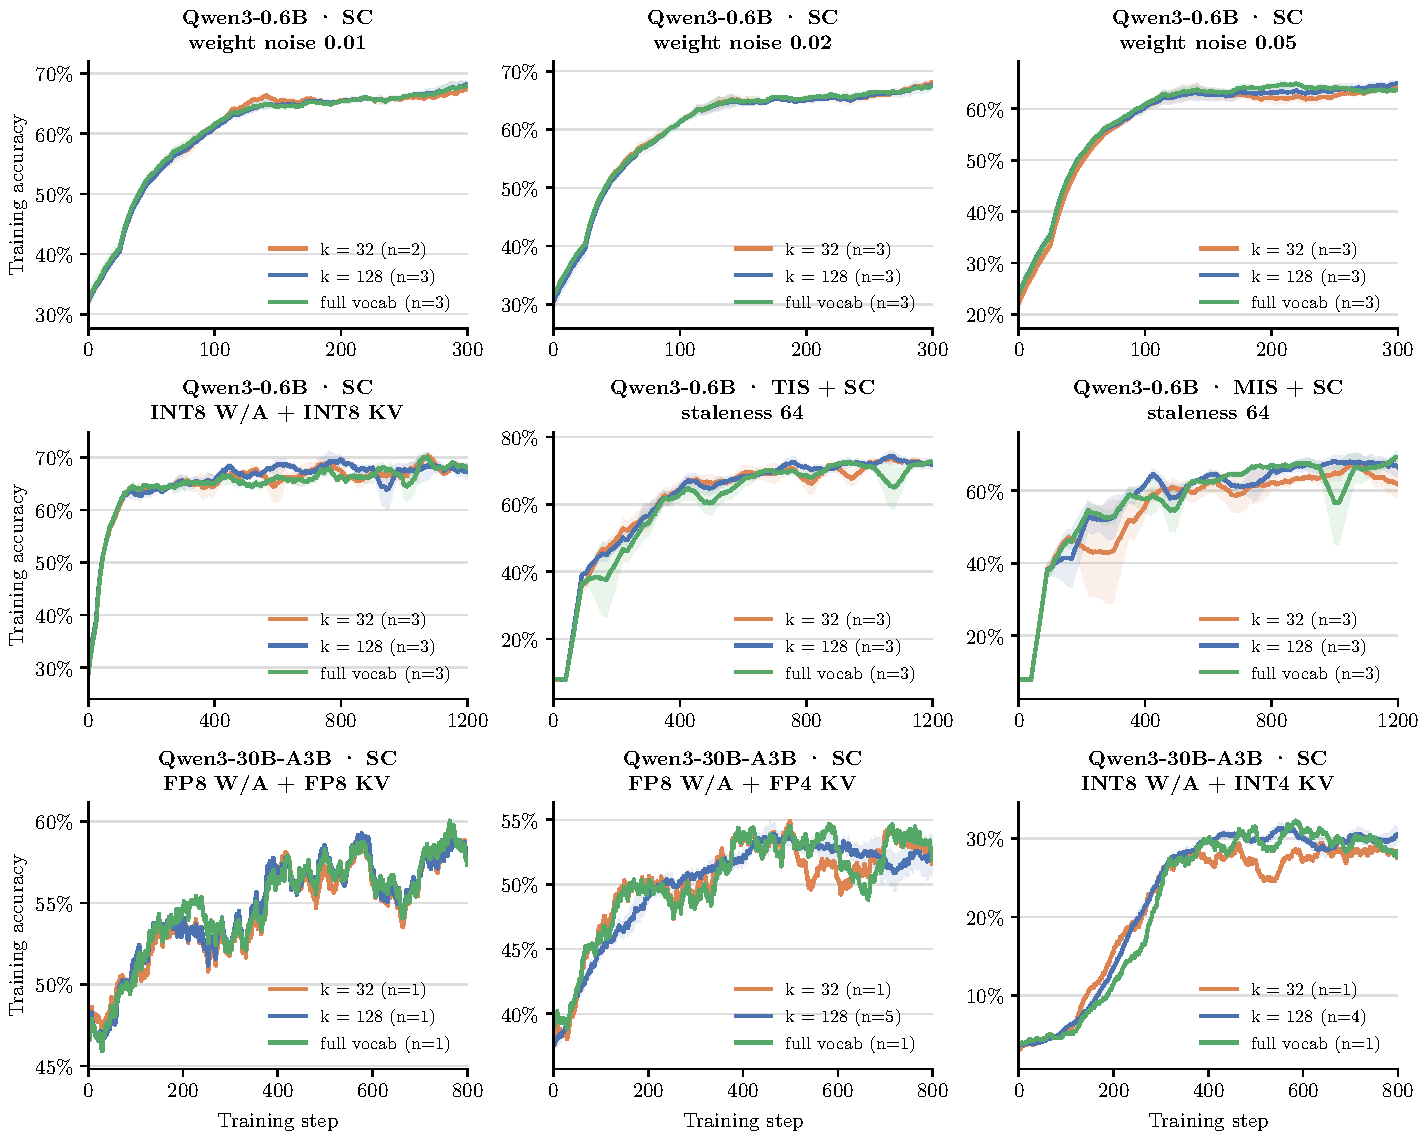
\includegraphics[width=1\linewidth]{plots/topk.pdf}
    \caption{Top-$k$  得分中心化消融实验。在所有测试情景中，使用 $k=128$  或 $k=32$  采样器的对数概率与 \Cref{eq:tail_model}  的尾部模型进行得分中心化，其效果与全词表得分中心化相当。每条曲线对应的种子数量显示在图例中。}
    \label{fig:top_k}
\end{figure}


\section{实验细节}
\label{sec:experimental_details}

\subsection{训练设置}

除非另有说明，我们使用以群体为中心奖励的REINFORCE：
\begin{equation}
J_{\mathrm{base}}(\theta)
= \frac{\sum_i A_i \sum_{t=1}^{L_i} \log p_\theta(y_{i,t}\mid y_{i,<t})}
       {\sum_i L_i},
\qquad A_i = R_i - \bar R_{\mathrm{group}},
\qquad R_i \in \{-1,+1\}.
\label{eq:shared_reinforce}
\end{equation}
这里 $i$  表示批量中的轨迹索引，$L_i$  表示轨迹长度，$\bar R_{\mathrm{group}}$  表示相同提示词的完成部分的平均奖励。

遵循~\citet{rl_sgd}，我们在所有实验中均使用SGD，学习率固定为$10^{-2}$。我们发现该学习率在所有实验中均表现稳定，且性能与AdamW相当，同时节省了高达240GB的内存。每个批量对每个提示采样8个完整序列，并执行一次优化器步骤。对于Countdown上的Qwen3-0.6B-Instruct，我们每批使用64个提示（共512个序列），最大序列长度为512；对于INTELLECT-2数学任务中的Qwen3-30B-A3B-Base，每批使用16个提示（共128个序列），最大序列长度为1024。更长的序列会增加TIM \citep{jet_rl}，但会使多个基准方法的多种子比较成本过高。

\subsection{修正方法}
\label{sec:is_methods}

我们比较的所有基于IS的方法都落在一个简单的网格上（\Cref{tab:is_methods}）。它们的区别在于修正操作是按token还是按序列进行，重要性比率是否被截断或掩码，以及修正哪些优势值的符号。DPPO使用基于二值总变差的掩码区域，而非重要性比率，但其目标函数仍使用IS权重。我们采用原始论文中的默认参数或\texttt{verl}的默认设置，未进行额外调优。所有重要性比率均相对于采样器记录的概率计算得出。GSPO使用原始论文中定义的token比率的几何平均值。

我们对同一目标应用每种修正，而不是从每篇论文中重新实现完整流程（\Cref{sec:results_setup}）。\Cref{tab:is_methods} 的最后一列提供了每种方法的实现细节。PG 使用 \Cref{eq:shared_reinforce} 而不进行任何修正。对于得分中心化，我们使用前-$k$ 的近似，并采用 $k=128$  (\Cref{sec:sc_implementation})。

\begin{table}[t]
    \centering
    \caption{基于IS的校正方法以表格形式表示，最后一列为实现说明。\texttt{Level} 决定统计量是按 token 还是按序列计算。\texttt{Outside} 指定在 \texttt{Low...High} 区域之外的行为。\texttt{Sign} 指定对哪些优势符号进行校正：\texttt{both} 将权重应用于每个 token；\texttt{neg} 仅对具有负优势的 token 应用（正优势 token 的权重保持为1）；\texttt{ppo} 应用 PPO 悲观截断，即加权目标与截断目标的极小点，因此截断仅在可能增大目标的方向上起作用。双截断遵循 \texttt{verl} 的 PPO 实现：比率高于 $3$  的负优势贡献被丢弃（对 GSPO 为整个响应）。$^{\mathrm P}$  表示论文默认设置，$^{\mathrm V}$  表示 \texttt{verl} 默认设置 \citep{verl}。}
    \label{tab:is_methods}
    \small
    \arrayrulecolor{gridline}
    \setlength{\arrayrulewidth}{0.3pt}
    \setlength{\tabcolsep}{3pt}
    \renewcommand{\arraystretch}{1.3}
    \begin{tabular}{@{}>{\raggedright\arraybackslash}m{70pt}
        >{\centering\arraybackslash}m{25pt}
        >{\centering\arraybackslash}m{24pt}
        >{\centering\arraybackslash}m{30pt}
        >{\centering\arraybackslash}m{30pt}
        >{\centering\arraybackslash}m{32pt}
        >{\centering\arraybackslash}m{22pt}
        >{\raggedright\arraybackslash}m{\dimexpr\linewidth-275pt\relax}@{}}
        \hline
        \rowcolor{gridgray}
        \textbf{Method} & \textbf{Level} & \textbf{Stat} & \textbf{Low} & \textbf{High} & \textbf{Outside} & \textbf{Sign} & \textbf{Implementation notes} \\
        \hline
        \cellcolor{gridgray}Naive IS \citep{reinforce} & \cellcolor{deep0!12}\texttt{token} & \cellcolor{tblteal!12}\texttt{ratio} & \cellcolor{deep1!50}0 & \cellcolor{deep1!50}$\infty$ & \cellcolor{gentlelilac!5}\texttt{-} & \cellcolor{deep2!30}\texttt{both} & --- \\
        \hline
        \cellcolor{gridgray}TIS$^{\mathrm V}$ \citep{tis}\par CISPO \citep{cispo} & \cellcolor{deep0!12}\texttt{token} & \cellcolor{tblteal!12}\texttt{ratio} & \cellcolor{deep1!50}0 & \cellcolor{deep1!30}2.0 & \cellcolor{gentlelilac!30}\texttt{clip} & \cellcolor{deep2!30}\texttt{both} & CISPO's dynamic sampling and length penalty omitted. \\
        \hline
        \cellcolor{gridgray}MIS (IcePop)$^{\mathrm P}$ \citep{icepop} & \cellcolor{deep0!12}\texttt{token} & \cellcolor{tblteal!12}\texttt{ratio} & \cellcolor{deep1!30}0.5 & \cellcolor{deep1!30}5.0 & \cellcolor{gentlelilac!10}\texttt{drop} & \cellcolor{deep2!30}\texttt{both} & Separate PPO surrogate between policy versions omitted. \\
        \hline
        \cellcolor{gridgray}PPO$^{\mathrm{P,V}}$ \citep{ppo} & \cellcolor{deep0!12}\texttt{token} & \cellcolor{tblteal!12}\texttt{ratio} & \cellcolor{deep1!16}0.8 & \cellcolor{deep1!16}1.2 & \cellcolor{gentlelilac!10}\texttt{drop} & \cellcolor{deep2!12}\texttt{ppo} & Dual clipping at $3$ (\texttt{verl} default). \\
        \hline
        \cellcolor{gridgray}DAPO$^{\mathrm{P,V}}$ \citep{dapo} & \cellcolor{deep0!12}\texttt{token} & \cellcolor{tblteal!12}\texttt{ratio} & \cellcolor{deep1!16}0.8 & \cellcolor{deep1!16}1.28 & \cellcolor{gentlelilac!10}\texttt{drop} & \cellcolor{deep2!12}\texttt{ppo} & Dual clipping at $3$; dynamic sampling and overlong reward penalty omitted. \\
        \hline
        \cellcolor{gridgray}GSPO$^{\mathrm{P,V}}$ \citep{gspo} & \cellcolor{deep0!38}\texttt{seq} & \cellcolor{tblteal!12}\texttt{ratio} & \cellcolor{deep1!6}0.9997 & \cellcolor{deep1!6}1.0004 & \cellcolor{gentlelilac!10}\texttt{drop} & \cellcolor{deep2!12}\texttt{ppo} & Token gradients summed rather than response-averaged; added dual clipping at $3$. \\
        \hline
        \cellcolor{gridgray}TOPR$^{\mathrm P}$ \citep{topr} & \cellcolor{deep0!38}\texttt{seq} & \cellcolor{tblteal!12}\texttt{ratio} & \cellcolor{deep1!50}0 & \cellcolor{deep1!6}1.0 & \cellcolor{gentlelilac!30}\texttt{clip} & \cellcolor{deep2!50}\texttt{neg} & --- \\
        \hline
        \cellcolor{gridgray}DPPO$^{\mathrm P}$ \citep{dppo} & \cellcolor{deep0!12}\texttt{token} & \cellcolor{tblteal!38}\texttt{tv} & \cellcolor{deep1!50}0 & \cellcolor{deep1!30}0.2 & \cellcolor{gentlelilac!10}\texttt{drop} & \cellcolor{deep2!12}\texttt{ppo} & No importance-ratio clipping. \\
        \hline
    \end{tabular}
\end{table}

\subsection{计算资源}

在所有图表中，阴影部分表示 $\pm 1$ 标准差。\Cref{fig:2b_online_vs_offline,fig:06b_weight_noise} 报告了在保留的评估提示上的准确率，而 \Cref{fig:30b_math,fig:06b_quant_stale,fig:top_k} 报告训练准确率，即采样轨迹的平均奖励，经过训练步数的中心移动平均平滑处理。

\Cref{tab:reproduction_compute} 列出了每种方法的种子数量以及重现每张图表所需的近似计算成本。

对于 0.6B 和 1.7B 模型，我们为每种修正方法（\Cref{fig:2b_online_vs_offline,fig:06b_weight_noise,fig:06b_quant_stale}）在每个实验中运行了 3 个种子。然而，由于训练 30B 模型（\Cref{fig:30b_math}）的成本高得多，我们最初仅以单个种子运行每种方法，之后仅对表现最佳的方法增加了更多种子（因为这些是我们最关心的对比）。在 FP8 KV 面板中，所有方法均为单种子；而在 FP4 KV 和 INT4 KV 面板中，分数中心化分别使用 5 和 4 个种子，TIS 使用 4 和 3 个，MIS 使用 3 和 3 个，而原始 IS 分别使用 2 和 1 个种子。

其余所有方法均为单种子。类似地，在 \Cref{fig:top_k} 中，$k=128$ 对于 30B 模型的结果来自 \Cref{fig:30b_math}，因此为多种子；$k=32$ 和完整分数中心化为单种子，以降低计算成本。

\begin{table}[H]
    \centering
    \caption{每条曲线的种子数及重现我们图表所需的近似计算量。实验主要在配备8$\times$ NVIDIA H100 SXM GPU的结点上运行。}
    \label{tab:reproduction_compute}
    \resizebox{\linewidth}{!}{%
    \arrayrulecolor{gridline}
    \setlength{\arrayrulewidth}{0.3pt}
    \begin{tabular}{lllrr}
        \hline
        \rowcolor{gridgray}
        \textbf{Experiment} & \textbf{Figure} & \textbf{Seeds} & \textbf{Unique runs} & \textbf{Approx. H100-hours} \\
        \hline
        \cellcolor{gridgray}Online vs.\ offline & \Cref{fig:2b_online_vs_offline} & 3 & 18 & 190 \\
        \hline
        \cellcolor{gridgray}Synthetic weight noise & \Cref{fig:06b_weight_noise} & 3 & 108 & 280 \\
        \hline
        \cellcolor{gridgray}Quantization and staleness & \Cref{fig:06b_quant_stale} & 3 & 72 & 1,120 \\
        \hline
        \cellcolor{gridgray}30B math & \Cref{fig:30b_math} & 1--5 & 47 & 3,750 \\
        \hline
        \cellcolor{gridgray}Top-$k$ ablation & \Cref{fig:top_k} & see legend & 51 & 840 \\
        \hline
        \cellcolor{gridgray}\textbf{Total} & & & \textbf{296} & \textbf{6,180} \\
        \hline
    \end{tabular}%
    }
\end{table}


\end{document}
